\subsection{Workflow dentro do Flux que utiliza das funções}

\subsubsection{Workflows BPL}

Os workflows laboratoriais de nome BPL (Boas Práticas de Laboratório) estavam separados em 5 workflows diferentes, já que existiam BPMs diferentes para cada tipo de usuário.
O problema com o BPL é que existem workflows pequenos (pouco profundos, com poucas atividades) e também existem workflows grandes (Com muitas atividades, profundos) e, com isso, surge a dificuldade de disponibilização de dados para diferentes tipos de usuários como a utilização do workflow por gerentes e técnicos de laboratório.

Essa dificuldade existe porque, para cada workflow, deve ser acessado uma página diferentes do LIMS, já que cada um desses workflows representa um sistema diferente para cada usuário.

Com a implementação de compartilhamento de informações entre workflows, conseguimos utilizar estes workflows junto a workflows diferentes para unirmos as boas práticas de laboratório aos workflows que a utilizam, tendo um maior controle de execução de cada um destes fluxos de trabalho, garantindo que todos estão seguindo as normas de BPL, como é o caso do CTTX.

% Para que esta ferramenta fosse mais poderosa, também foi implementado a funcionalidade de múltiplas atividades iniciais no workflow do BPL, fazendo com que workflows dinâmicos pudessem ser centralizados em qualquer atividade que estivesse compartilhada entre instâncias, agregando informações necessárias para execução de um BPM, como calibração de um equipamento de análise de substâncias.

\subsubsection{CTTX e BPL - Equipamentos}

O workflow de Citotoxicidade (CTTX) utiliza o workflow \textit{BPL - Equipamentos} para garantir que equipamentos estejam calibrados e funcionais. Uma atividade deste workflow só deve ser executada quando as calibrações dos equipamentos utilizados estiverem em dia.

Para isso, foi compartilhada a atividade de calibração do workflow \textit{BPL - Equipamentos} com o workflow \textit{CTTX}, implementando este fluxo de trabalho no Flux, adaptando o workflow para que atividades do workflow CTTX apenas estivessem disponíveis para execução após uma calibração.

A estrutura dentro do Flux fica demonstrada pela figura~\ref{fig:cttx_bpl_flux}, que pode ser acessada dentro do próprio software. Na figura, podemos ver referência à atividade ``Calibração" nos dois fluxos de trabalho. Para separar quais atividades ficam disponíveis para cada usuário do sistema, é necessário utilizar o sistema de permissões já implementado no Flux para especificar permissões de visualização, execução e aprovação da atividade.

\begin{figure}
    \centering
    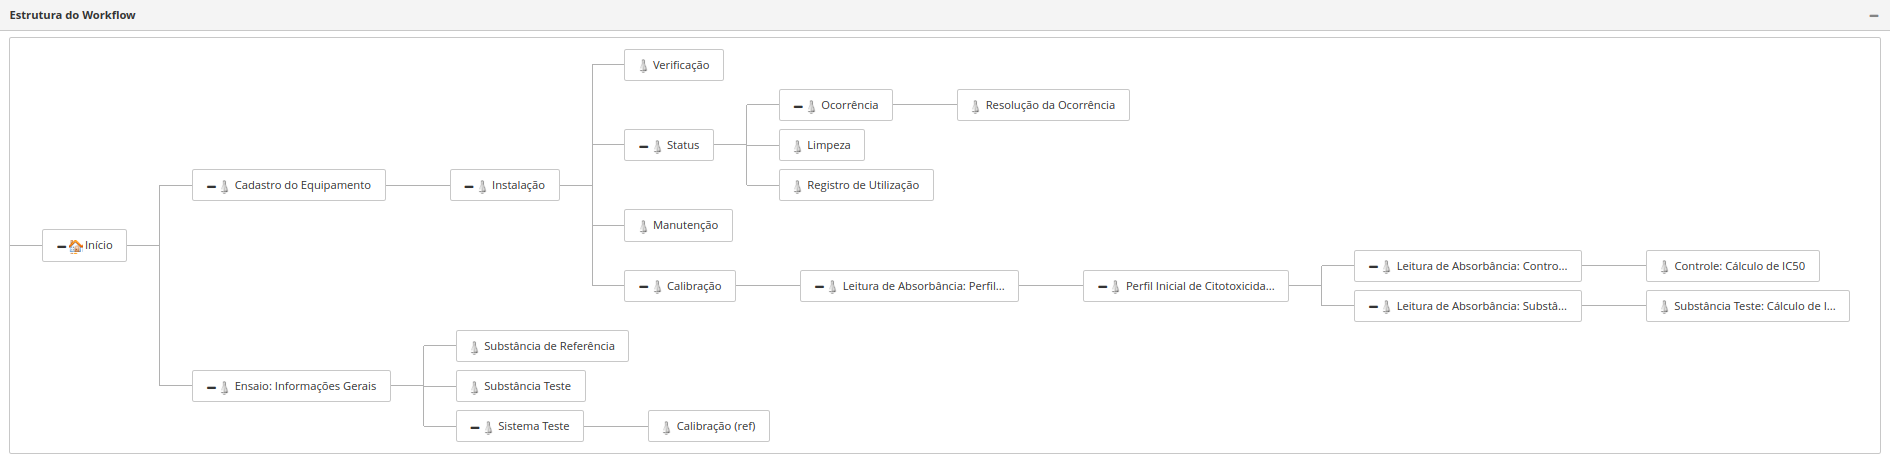
\includegraphics[width=1\textwidth]{imgs/CTTX-EQP/estrutura_cttx_eqp_flux.png}
    \caption{Estrutura do workflow conjunto CTTX com BPL - Equipamentos demonstrada pela interface do Flux. Como podemos ver pela imagem, após a atividade ``Sistema teste" (canto inferior da imagem), temos a atividade ``Calibração (ref)", que refere-se a atividade calibração no fluxo de trabalho demonstrado logo acima.}
    \label{fig:cttx_bpl_flux}
\end{figure}

Assim, podem ser separados usuários que irão executar a atividade de calibração do equipamento de usuários que irão realizar os experimentos a partir daquela calibração, diminuindo os erros que podem ocorrer caso as atividades sejam disponibilizadas sem que um equipamento tenha sido calibrado corretamente.

Na visão de um administrador, podemos ver pelo software que a mesma atividade selecionada de calibração foi realizada, e as mesmas atividades são disponibilizadas para o usuário (Por ele ter permissão de ver todas as atividades) de maneira automática com o compartilhamento de atividades, visto nas figuras~\ref{fig:cttx_executado_calibracao_equipamento} e~\ref{fig:cttx_executado_calibracao_leitura_absorbancia}.

\begin{figure}
    \centering
    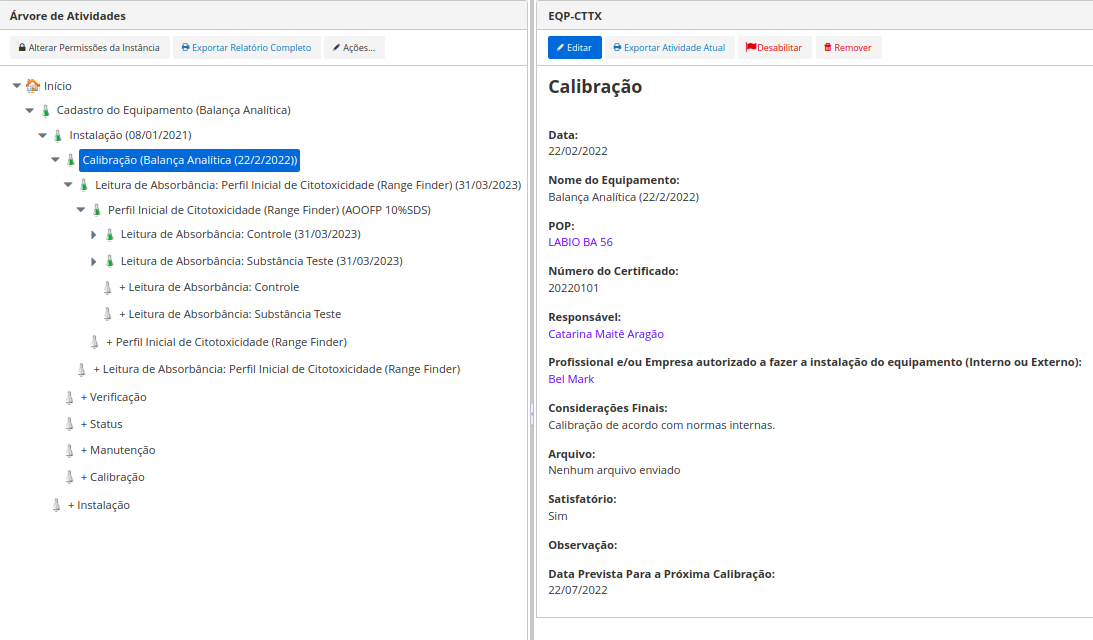
\includegraphics[width=0.7\textwidth]{imgs/CTTX-EQP/cttx_executado_calibracao_equipamento.png}
    \caption{Atividade de calibração executada seguindo o workflow de cadastro de equipamento, seguindo o cadastro e a instalação do mesmo. Podemos ver que a atividade de calibração é a mesma da figura~\ref{fig:cttx_executado_calibracao_leitura_absorbancia}}
    \label{fig:cttx_executado_calibracao_equipamento}
\end{figure}

\begin{figure}
    \centering
    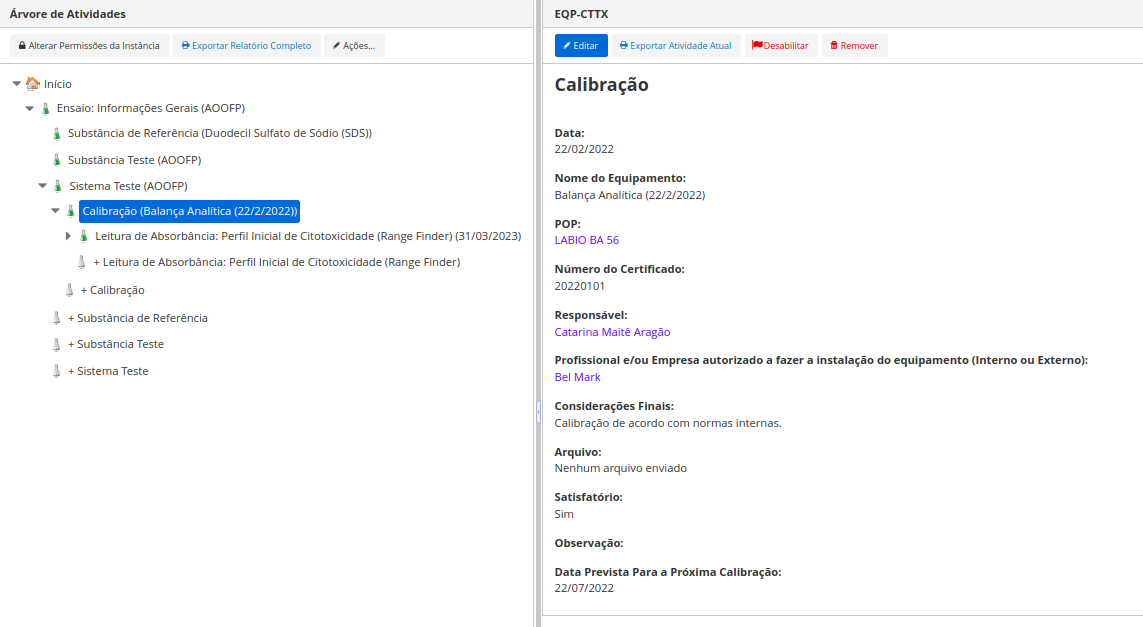
\includegraphics[width=0.7\textwidth]{imgs/CTTX-EQP/cttx_executado_calibracao_ensaio.png}
    \caption{Atividade de calibração executada seguindo o workflow de ensaio, que analisa as amostras. Podemos ver que a atividade de calibração é a mesma da figura~\ref{fig:cttx_executado_calibracao_equipamento}}
    \label{fig:cttx_executado_calibracao_leitura_absorbancia}
\end{figure}